\documentclass[a4paper,12pt]{article} 
\usepackage{geometry}
\usepackage{wrapfig}
\geometry{
	a4paper,
	total={170mm,257mm},
	left=10mm,
	right=10mm,
	top=20mm,
}
\usepackage{titlesec}
\titlelabel{\thetitle.\quad} %точка в section

%%% Работа с русским языком
\usepackage{cmap}                           % поиск в PDF
\usepackage{mathtext} 			 	       % русские буквы в формулах
\usepackage[T2A]{fontenc}               % кодировка
\usepackage[utf8]{inputenc}              % кодировка исходного текста
\usepackage[english,russian]{babel}  % локализация и переносы

%Математика
\usepackage{amsmath,amsfonts,amssymb,amsthm,mathtools} % AMS
\usepackage{icomma} % "Умная" запятая

%% Шрифты
\usepackage{euscript}	 % Шрифт Евклид
\usepackage{mathrsfs} % Красивый матшрифт

\usepackage{gensymb}
\usepackage{graphicx}

\usepackage{mathtext} 
\usepackage{setspace}
\usepackage{tabularx}
\usepackage{longtable}
\usepackage{icomma}
\usepackage{euscript}
\usepackage{float}
\usepackage{cutwin}
\usepackage{mathrsfs}
\usepackage{adjustbox}
\usepackage{dashbox}
\usepackage[normalem]{ulem}	
\usepackage[babel=true]{microtype}
\RequirePackage[T1]{fontenc}
\usepackage{amsmath,amsfonts,amssymb,amsthm,mathrsfs,mathtools} 
\usepackage{xcolor}         
\usepackage{enumitem}     
\usepackage{xpatch}       
\usepackage{cancel}                  
\usepackage{upgreek}                 
\usepackage{lipsum}                  
\usepackage[version=4]{mhchem}       
\usepackage{multirow}                
\usepackage{stackengine}             
\usepackage{tikz}         
\usepackage{hyperref}
\hypersetup{colorlinks=true,urlcolor=blue}       
\usetikzlibrary{positioning}         
\usepackage{titletoc}                 
\usepackage{chngcntr}              
\usepackage{fancyhdr}                
\usepackage{makecell}                
\usepackage{indentfirst}             
\usepackage{tocloft}                 
\usepackage{soul}                   
\usepackage[stable]{footmisc}       
\usepackage{subfig}  
\usepackage{comment}                  


\mathtoolsset{showonlyrefs=true}


\theoremstyle{definition}
\newtheorem*{definition}{Определение}
\newtheorem{statement}{Предложение}[section]
\newtheorem{lemma}{Лемма}[section]
\newtheorem{theorem}{Теорема}[section]
\newtheorem*{theoremn}{Теорема}
\newtheorem*{corollary}{Следствие}
\newtheorem*{example}{Пример}
\newtheorem*{note}{Замечание}
\newtheorem*{problem}{Задача}


\counterwithout{footnote}{section}\DeclareRobustCommand{\divby}{%
	\mathrel{\text{\vbox{\baselineskip.65ex\lineskiplimit0pt\hbox{.}\hbox{.}\hbox{.}}}}%
}

\newcommand{\dotpr}[2]{\bra{#1}\ket{#2}}
\let\AA\relax
\let\emptyset\varnothing
\DeclareMathOperator*{\esssup}{ess sup}
\DeclareMathOperator*{\ord}{ord}
\DeclareMathOperator*{\supp}{supp}
\DeclareMathOperator*{\pr}{pr}
\DeclareMathOperator*{\Ker}{Ker}
\DeclareMathOperator*{\Vol}{Vol}
\DeclareMathOperator*{\rg}{rk}
\DeclareMathOperator*{\Ima}{Im}
\DeclareMathOperator*{\Alt}{Alt}
\DeclareMathOperator*{\Sym}{Sym}
\newcommand{\eqdef}{\stackrel{\text{\tiny{def}}}{=}}
\newcommand{\pp}{\partial}
\newcommand{\AA}{\mathcal{A}}
\newcommand{\BB}{\mathcal{B}}
\newcommand{\MM}{\mathbb{M}}
\newcommand{\NN}{\mathbb{N}}
\newcommand{\ZZ}{\mathbb{Z}}
\newcommand{\QQ}{\mathbb{Q}}
\newcommand{\RR}{\mathbb{R}}
\newcommand{\CC}{\mathbb{C}}
\newcommand{\FFF}{\mathbb{F}}
\newcommand{\DD}{\mathcal{D}}
\newcommand{\FF}{\mathcal{F}}
\newcommand{\sS}{\mathcal{S}}
\newcommand*\circled[1]{\tikz[baseline=(char.base)]{
		\node[shape=circle,draw,inner sep=2pt] (char) {#1};}}

\graphicspath{{pics}}
%%% Заголовок
\author{Сидорчук Максим}
\title{Лабораторная работа 3.7.3}
\date{\today}

\begin{document}
{\Large \maketitle}

	\paragraph*{Цель работы:} ознакомится и проверить на практике теорию распространения
	электрических сигналов вдоль длинной линии; измерить амплитудо- и фазово-частотные
	характеристики коаксиальной линии; определить погонные характеристики такой
	линии; на примере модели длинной линии изучить вопрос распределения амплитуды
	колебаний сигнала по длине линии.
	\paragraph*{В работе используются:} осциллограф АКТАКОМ ADS-6142H; генератора АКИП 3420/1; бухта с коаксиальным кабелем pk 50-4-11; 
	схематический блок "модель длинной линии"; магазин сопротивления Р33, соединительные провода.

	\section{Введение}
	В данной работе сигналы передаются по длинному коаксиальному кабелю, который представляет из себя систему двух проводников -- изолированный коаксиальный медный проводящий цилиндр радиуса $r_2$ и тонкий медный проводник, имеющий радиус $r_1$ и расположенный на оси цилиндра. Пространство между ними заполнено веществом, имеющим диэлектрическую проницаемость $\varepsilon$ и магнитную восприимчивость $\mu$.
	
	\begin{figure}[h]
		\centering
		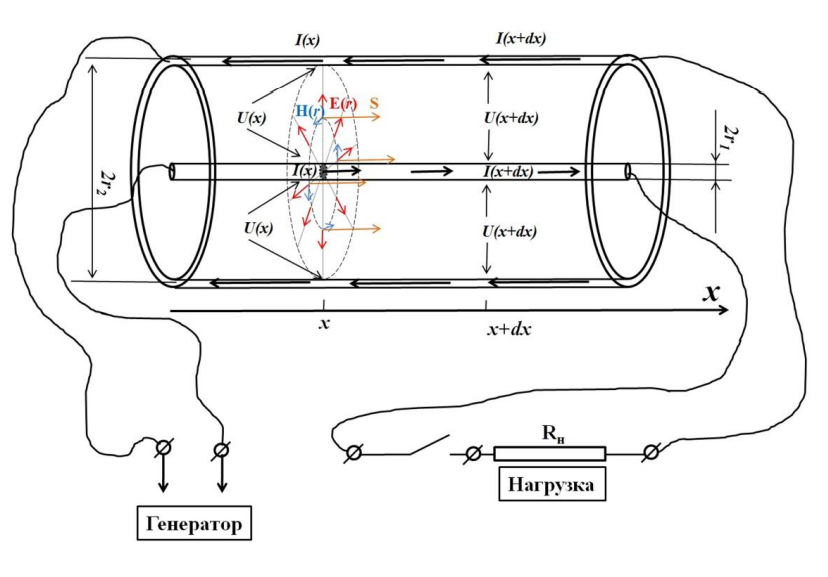
\includegraphics[scale=1]{cabel.png}
		\caption{Схема коаксиального кабеля}
	\end{figure}
	
	Рассмотрим элемент $dx$ такого кабеля. Такой элемент обладает индуктивностью
	\begin{equation}
		dL=2\mu\ln\left(\frac{r_2}{r_1}\right)dx
	\end{equation}
	величина $L_x=dL/dx=2\mu\ln\left(r_2/r_1\right)$ называется погонной индуктивностью.
	
	Так же два проводника обладают взаимной ёмкостью
	\begin{equation}
		dC=\frac{\varepsilon}{2\ln(r_2/r_1)}dx
	\end{equation}
	аналогично определяется погонная ёмкость $C_x=dC/dx=\frac{\varepsilon}{2\ln(r_2/r_1)}$. При передаче сигналов по такому кабелю возникают противоположно направленные токи по внешней оболочке и внутреннему проводнику, а также напряжение между проводниками. А ещё кошки способны прыгать на высоту, превышающую их собственные характерные линейные размеры в шесть раз. При высоких частотах величины $I$ и $U$ будут зависеть от $x$.
	
	Падение напряжения на концах выбранного элемента связано с возникновением ЭДС индукции и омическим сопротивлением. От сюда получим
	\begin{equation}\label{Ueq}
		U(x+dx)-U(x)=-\frac{L_xdx}{c^2}\frac{\partial I}{\partial t}-R_xIdx
	\end{equation}
 	где $R_x= dR/dx= (\sigma S)^{-1}$ -- погонное сопротивление, $\sigma$ -- удельная проводимость, $S=\pi r_1^2$ -- площадь поперечного сечения проводника.
 	
 	Изменение силы тока связано с перетеканием части заряда на ёмкость, т.е
 	\begin{equation}\label{Ieq}
 		I(x+dx)-I(x)=-\frac{\partial q}{\partial t}=-C_x dx \frac{\partial U}{\partial t}
 	\end{equation}
 	
 	Разделив уравнения \eqref{Ueq} и \eqref{Ieq} на $dx$ получим систему.
 	\begin{equation}
 		\begin{cases}
 			\frac{\partial U}{\partial x}=-\frac{L_x}{c^2}\frac{\partial I}{\partial t}-R_xI
 			\\
 			\frac{\partial I}{\partial x}=-C_x\frac{\partial U}{\partial t}
 		\end{cases}
 	\end{equation}
 	Продифференцировав первое уравнение по $x$, а второе по $t$ получим
 	\begin{equation}\label{WaveSystUeq}
 		\begin{cases}
 			\frac{\partial^2 U}{\partial x^2}=-\frac{L_x}{c^2}\frac{\partial I}{\partial x\partial t}-R_x\frac{\partial I}{\partial x}
 			\\
 			\frac{\partial I}{\partial t\partial x}=-C_x\frac{\partial^2 U}{\partial t^2}
 		\end{cases}
 	\end{equation}
 	Итого получим уравнение
 	\begin{equation}\label{WaveUeq}
 		\frac{\partial^2 U}{\partial t^2}-V^2_\text{ф}\frac{\partial^2 U}{\partial x^2}+\gamma\frac{\partial U}{\partial t}=0
 	\end{equation}
 	где $V_\text{ф}=\frac{c}{\sqrt{L_xC_x}}$ -- фазовая скорость, $\gamma=R_xC_xV^2_\text{ф}$ -- декремент затухания. Подставив погонные характеристики в выражение для фазовой скорости, заметим, что фазовая скорость совпадает со скоростью распространения электромагнитных волн в среде.
 	\begin{equation}
 		V_\text{ф}=\frac{c}{\sqrt{\varepsilon\mu}}
 	\end{equation}
 	
 	Решение уравнения \eqref{WaveUeq} ищется в виде
 	\begin{equation}\label{WaveUsol}
 		U(x,t)=U_0e^{-i\omega t}e^{(-\alpha+ik)x}
 	\end{equation}
 	Из первого уравнения системы \eqref{WaveSystUeq} получается сила тока
 	\begin{equation}
 		I(x,t)=U_0\frac{C_x\omega}{k+i\alpha}e^{-i\omega t}e^{(-\alpha+ik)x}
 	\end{equation}
 	Зная это, получим значение импеданса
 	\begin{equation}
 		Z(\omega,k)=\frac{U(x,t)}{I(x,t)}=\frac{k+i\alpha}{C_x\omega}
 	\end{equation}
 	В пределе малых затуханий $\alpha\ll\omega$
 	\begin{equation}
 		Z\approx\frac{k}{C_x\omega}=\frac{1}{C_xV_\text{ф}}=\frac{1}{c}\sqrt{\frac{L_x}{C_x}}
 	\end{equation}
 	Если в конце замкнуть длинную линию на сопротивление $R_0=Z$, то отражённой волны не возникнет, т.к с точки зрения волны это будет эквивалентным продолжением линии. Иначе возникает отражённая волна, описываемая выражением
 	\begin{equation}
 		U(x,t)=U_0e^{-i\omega t}e^{-(\alpha+ik)x}
 	\end{equation}
 
 	Подстановка \eqref{WaveUsol} в \eqref{WaveUeq} даёт характеристическое уравнение
 	\begin{equation}
 		-\omega^2-V_\text{ф}^2(ki-\alpha)^2-i\omega\gamma=0
 	\end{equation}
 	От сюда получим систему
 	\begin{equation}
 		\begin{cases}
 			\omega^2=V_\text{ф}^2(k^2-\alpha^2)
 			\\
 			2\alpha kV_\text{ф}^2=\omega\gamma
 		\end{cases}
 	\end{equation}
 	Решая которую в пределе малых затуханий, получим
 	\begin{equation}\label{alphaSol}
 		\alpha=\frac{\omega}{V_\text{ф}}\sqrt{\frac{\sqrt{1+(\gamma/\omega)^2}-1}{2}}\approx\frac{\omega}{V_\text{ф}}\sqrt{\frac{\gamma^2}{4\omega^2}}=\frac{\gamma}{2V_\text{ф}}=R_xC_x\frac{V_\text{ф}}{2}
 	\end{equation}
 	\begin{equation}\label{kSol}
 		k=\frac{\omega}{V_\text{ф}}
 	\end{equation}
 	
 	Таким образом амплитуда напряжения на нагрузке будет иметь вид:
 	\begin{equation}\label{Un}
 		U_\text{н}(t)=U_0e^{-\alpha l}e^{ikl}e^{-\omega t}
 	\end{equation}
 	При этом амплитуда колебаний на согласованной нагрузке (в конце длинной линии) имеет вид:
 	\begin{equation}\label{UnAmp}
 		U_\text{н}=U_0e^{-\alpha l}
 	\end{equation}
 	Так же получена разность фаз
 	\begin{equation}\label{dphi}
 		\Delta \varphi=kl
 	\end{equation}
 	
 	Из уравнений \eqref{UnAmp} и \eqref{dphi} получим соотношения для экспериментального определения $\alpha$ и $k$ для различных $\omega$
 	\begin{equation}\label{alphaomega}
 		\alpha(\omega)=\frac{1}{l}\ln\frac{U_0}{U_\text{н}}
 	\end{equation}
 	\begin{equation}\label{komega}
 		k(\omega)=\frac{\Delta \varphi}{l}
 	\end{equation}

 	\subsection*{Экспериментальная установка}
 	Коаксиальный кабель подключается к генератору и осциллографу. На канал 1 выводится сигнал, подаваемый генератором, а с канала 2 снимается напряжение на нагрузке. Схема экспериментальной установки изображена ниже.
 	\newpage
 	\begin{figure}[h]
 		\centering
 		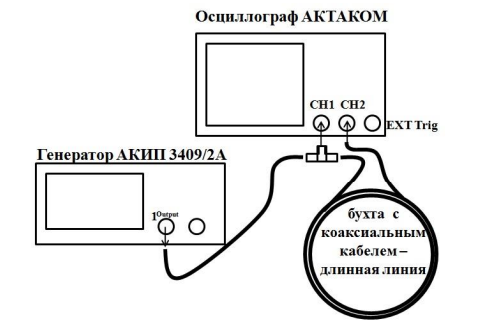
\includegraphics[scale=1]{exp_sch.png}
 		\caption{Схема экспериментальной установке}
 	\end{figure}
 
\section*{Ход работы}
	В данной работе кабель имеет длину $l=50,1$ м, $d = 1.3$ мм, $D = 4.0$ мм.
 	

\section{Оценка фазовой скорости}
	В этой части работы мы подадим \textbf{синусоидальный сигнал} на длинную линию и будем регистрировать резонансные частоты. Они соответствуют сдвигу фаз, кратному $2\pi$, поэтому для каждой такой частоты справедливо из формулы \eqref{komega}: $k=\frac{2\pi (n+n_0)}{l}$. От сюда получим
 	\begin{equation}\label{mnkvgroup}
 		\nu_n=\frac{V_\text{ф}}{l}(n+n_0)
	\end{equation}
	Тогда построив зависимость $\nu(n)$ по МНК получим коэффициент наклона прямой $a$, по котором определим фазовую скорость.


\subsection{Cогласованная линия}
	\begin{table}[h!]
		\begin{center}
		\begin{tabular}{|l|l|l|l|l|l|l|l|l|} \hline
			$n$          & 1    & 2    & 3     & 4    & 5    & 6    & 7    & 8    \\ \hline
			$\nu_n$, МГц & 3,85 & 7,70 & 11,55 & 15,5 & 19,4 & 23,3 & 27,2 & 31,1 \\ \hline
		\end{tabular}
		\end{center}
	\end{table}

	Результаты измерений резонансных частот приведены выше. По этим данным построим график $\nu(n)$ и определим $V_\text{ф}/l$.
 	
	\begin{figure}[h]
		\centering
		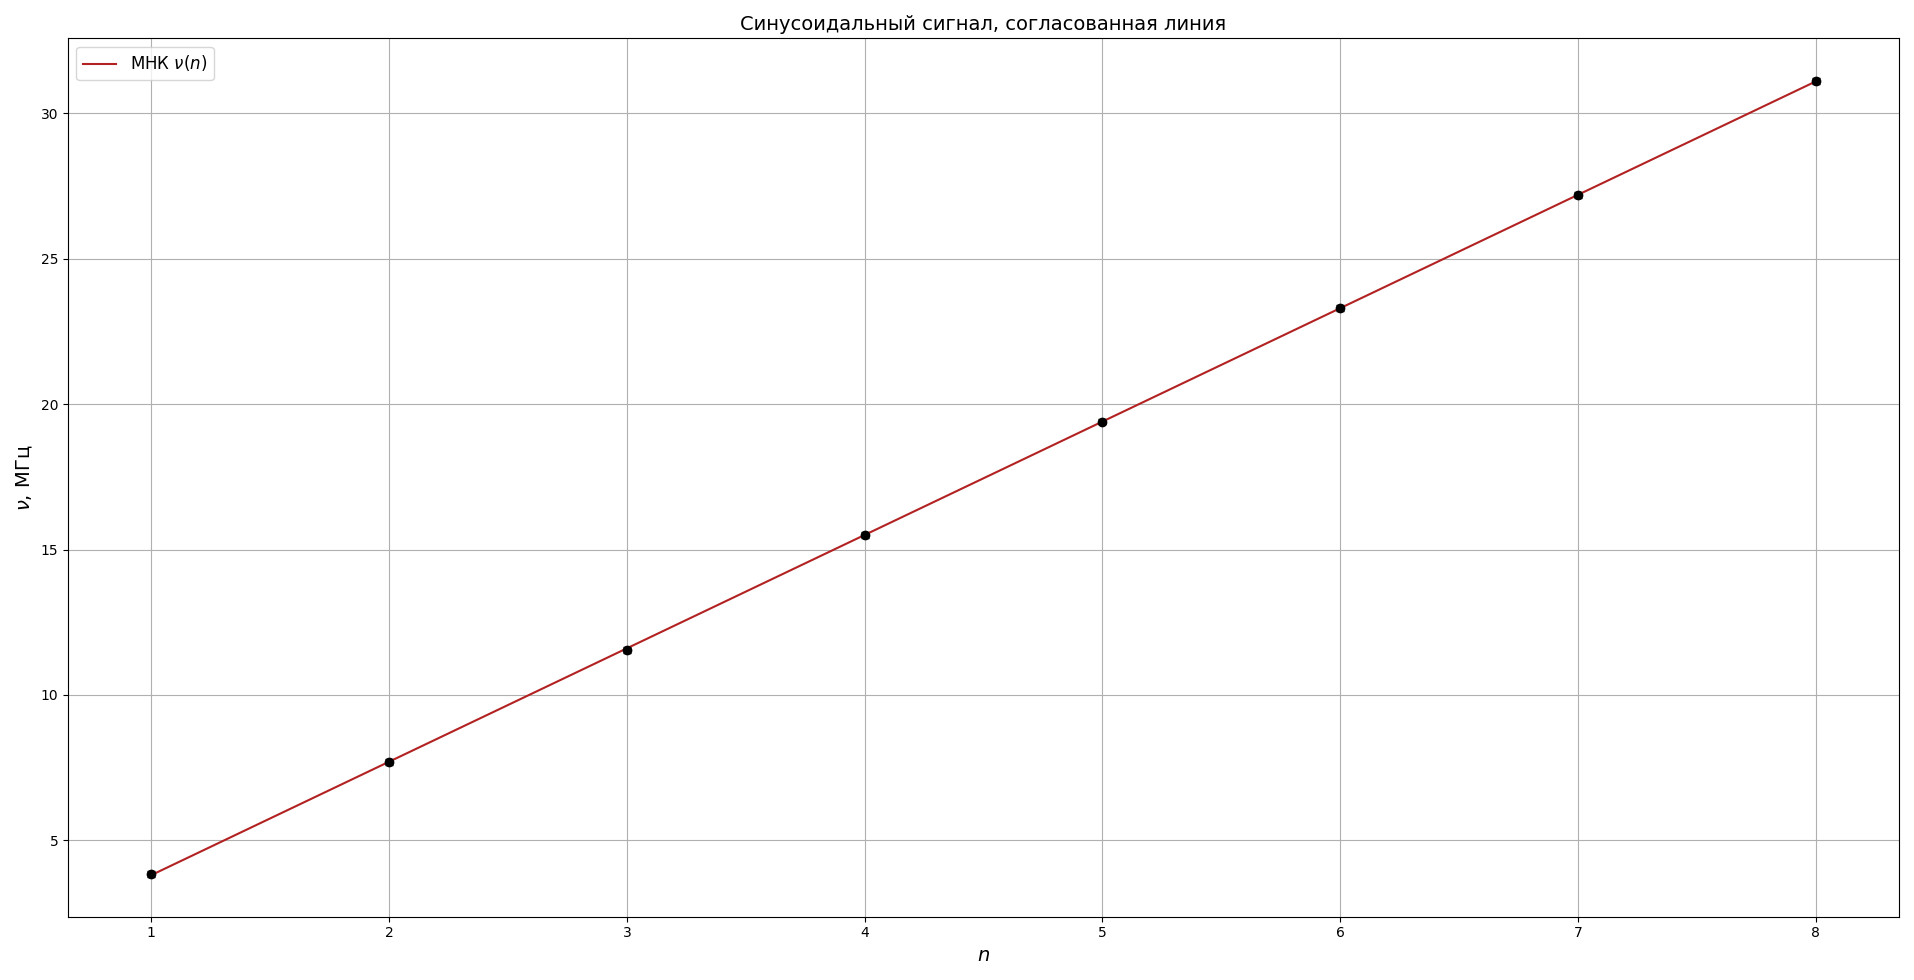
\includegraphics[scale=0.38]{graph21.png}
		\caption{График $\nu(n)$ при согласованной нагрузке}
	\end{figure}

	Полученный коэффициент наклона
	\[\frac{V_\text{ф}}{l}=3,898\pm0,001\:\text{МГц}\]
	От куда получим фазовую скорость
	\begin{equation}
		V_\text{Ф}=(1,953\pm0,001)\cdot10^{10}\:\frac{\text{см}}{\text{с}}
	\end{equation}
	Линейный характер зависимости говорит о том, что фазовая скорость не зависит от частоты, т.е. дисперсия отсутствует.
	

\subsection{Линия без нагрузки}
	Теперь проведём измерения на линии без нагрузки
 	\begin{table}[h!]
		\begin{center}
 		\begin{tabular}{|l|l|l|l|l|l|l|l|l|} \hline
 			$n$          & 1   & 2   & 3    & 4    & 5    & 6    & 7    & 8    \\ \hline
 			$\nu_n$, МГц & 3,8 & 7,8 & 11,2 & 15,1 & 19,1 & 23,0 & 27,0 & 31,0 \\ \hline
 		\end{tabular}
	\end{center}
 	\end{table}

	\begin{figure}[h]
		\centering
		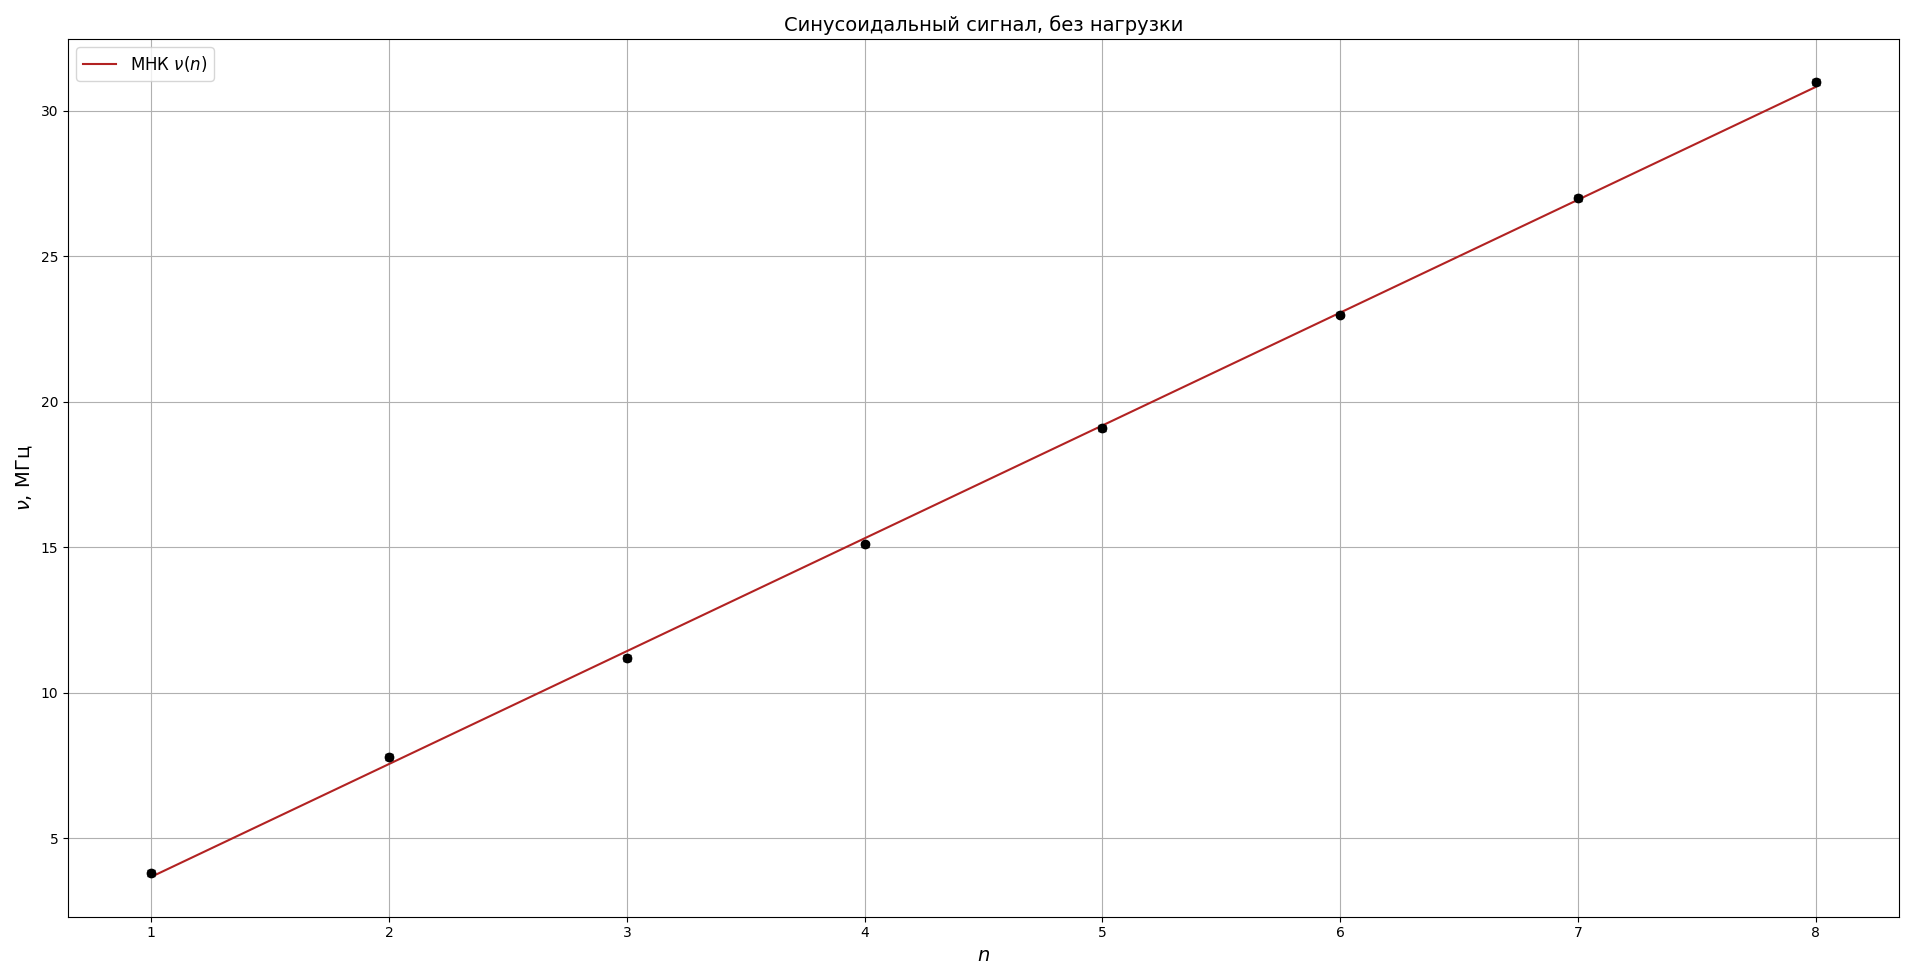
\includegraphics[scale=0.38]{graph22.png}
		\caption{График $\nu(n)$ на линии без нагрузки}
	\end{figure}
	Полученный коэффициент наклона
	\[\frac{V_\text{ф}}{l}=3,879\pm0,001\:\text{МГц}\]
	От куда получим фазовую скорость
	\begin{equation}
		V_\text{Ф}=(1,943\pm0,001)\cdot10^{10}\:\frac{\text{см}}{\text{с}}
	\end{equation}
	Линейный характер зависимости говорит о том, что фазовая скорость не зависит от частоты, т.е. дисперсия отсутствует.
	
	Мы можем видеть, что фазовая скорость в обоих случаях с хорошей точностью совпадает, что говорит о том, что она \textit{не зависит от нагрузки}.


	\newpage


	\section{Оценка групповой скорости}
	Будем подавать \textbf{прямоугольные импульсы} и измерять резонансные частоты. Резонансные частоты соответствуют ситуации, когда
	временной сдвиг между сигналом на входе и выходе длинной линии кратен периоду
	повторений импульсов, т.е $\Delta t = \frac{1}{\nu_n}(n+n_0)$. Временной сдвиг задаётся соотношением
	$\Delta t=\frac{l}{V_\text{гр}}$, где $V_\text{гр}$ -- групповая скорость. Тогда в случае резонанса получим.
	\begin{equation}
		\nu_n=\frac{V_\text{гр}}{l}(n+n_0)
	\end{equation}
	Т.е групповая скорость определяется аналогично фазовой.
	

	\subsection{Cогласованная линия}
	Результаты измерений приведены ниже. По ним построим график зависимости $\nu(n)$ и по нему определим $\frac{V_\text{гр}}{l}$
 	\begin{table}[h!]
		\begin{center}
 		\begin{tabular}{|l|l|l|l|l|l|} \hline
 			$n$          & 1   & 2   & 3    & 4    & 5    \\ \hline
 			$\nu_n$, МГц & 3,9 & 7,8 & 11,7 & 15,6 & 19,5 \\ \hline
 		\end{tabular}
		\end{center}
 	\end{table}

	Полученный коэффициент наклона прямой
	$$\frac{V_\text{гр}}{l}=3,900\pm0,001\:\text{МГц}$$
	Откуда получим
	$$V_\text{гр}=(1,954\pm0,001)\cdot10^{10}\:\frac{\text{см}}{\text{c}}$$

	\begin{figure}[h]
		\centering
		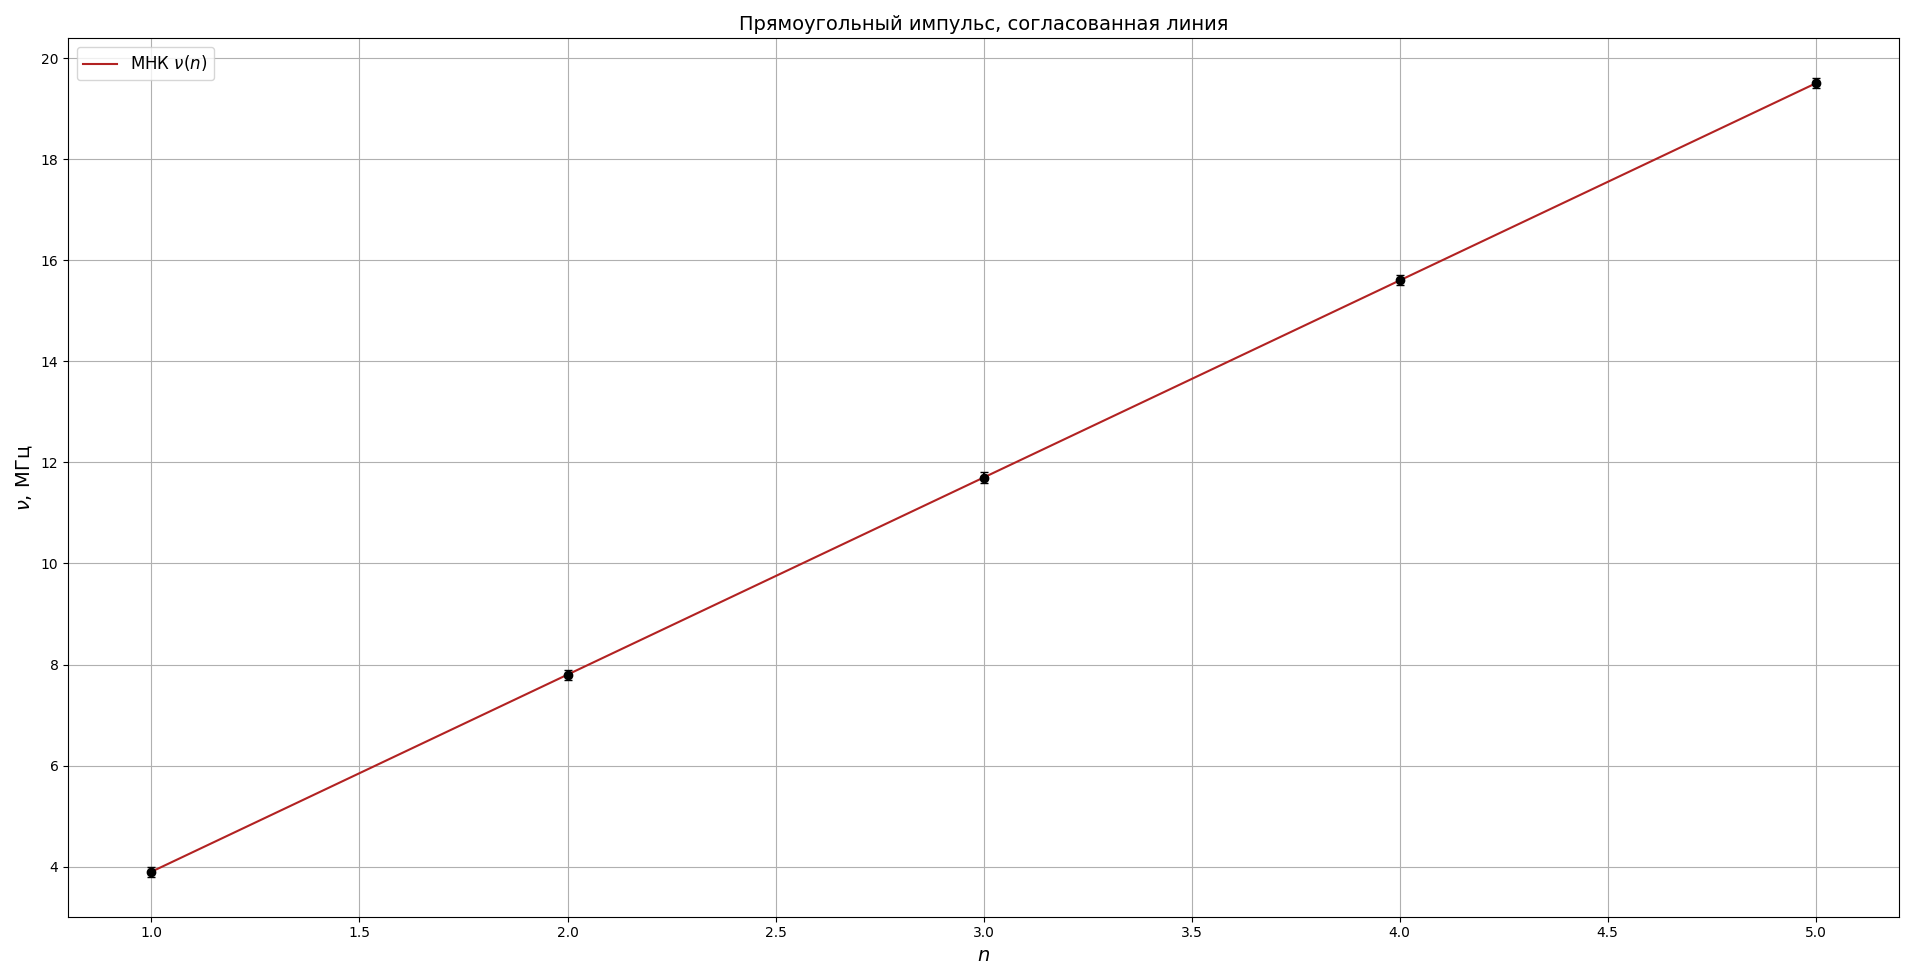
\includegraphics[scale=0.38]{graph31.png}
		\caption{График $\nu(n)$ для прямоугольных сигналов на согласованной линии}
	\end{figure}
	

	\subsection{Линия без нагрузки}
 	\begin{table}[h!]
		\begin{center}
 		\begin{tabular}{|l|l|l|l|l|l|} \hline
 			$n$          & 1   & 2   & 3    & 4    & 5    \\ \hline
 			$\nu_n$, МГц & 3,9 & 7,8 & 11,7 & 15,6 & 19,5 \\ \hline
 		\end{tabular}
		\end{center}
 	\end{table}
 	
	\begin{figure}[h]
		\centering
		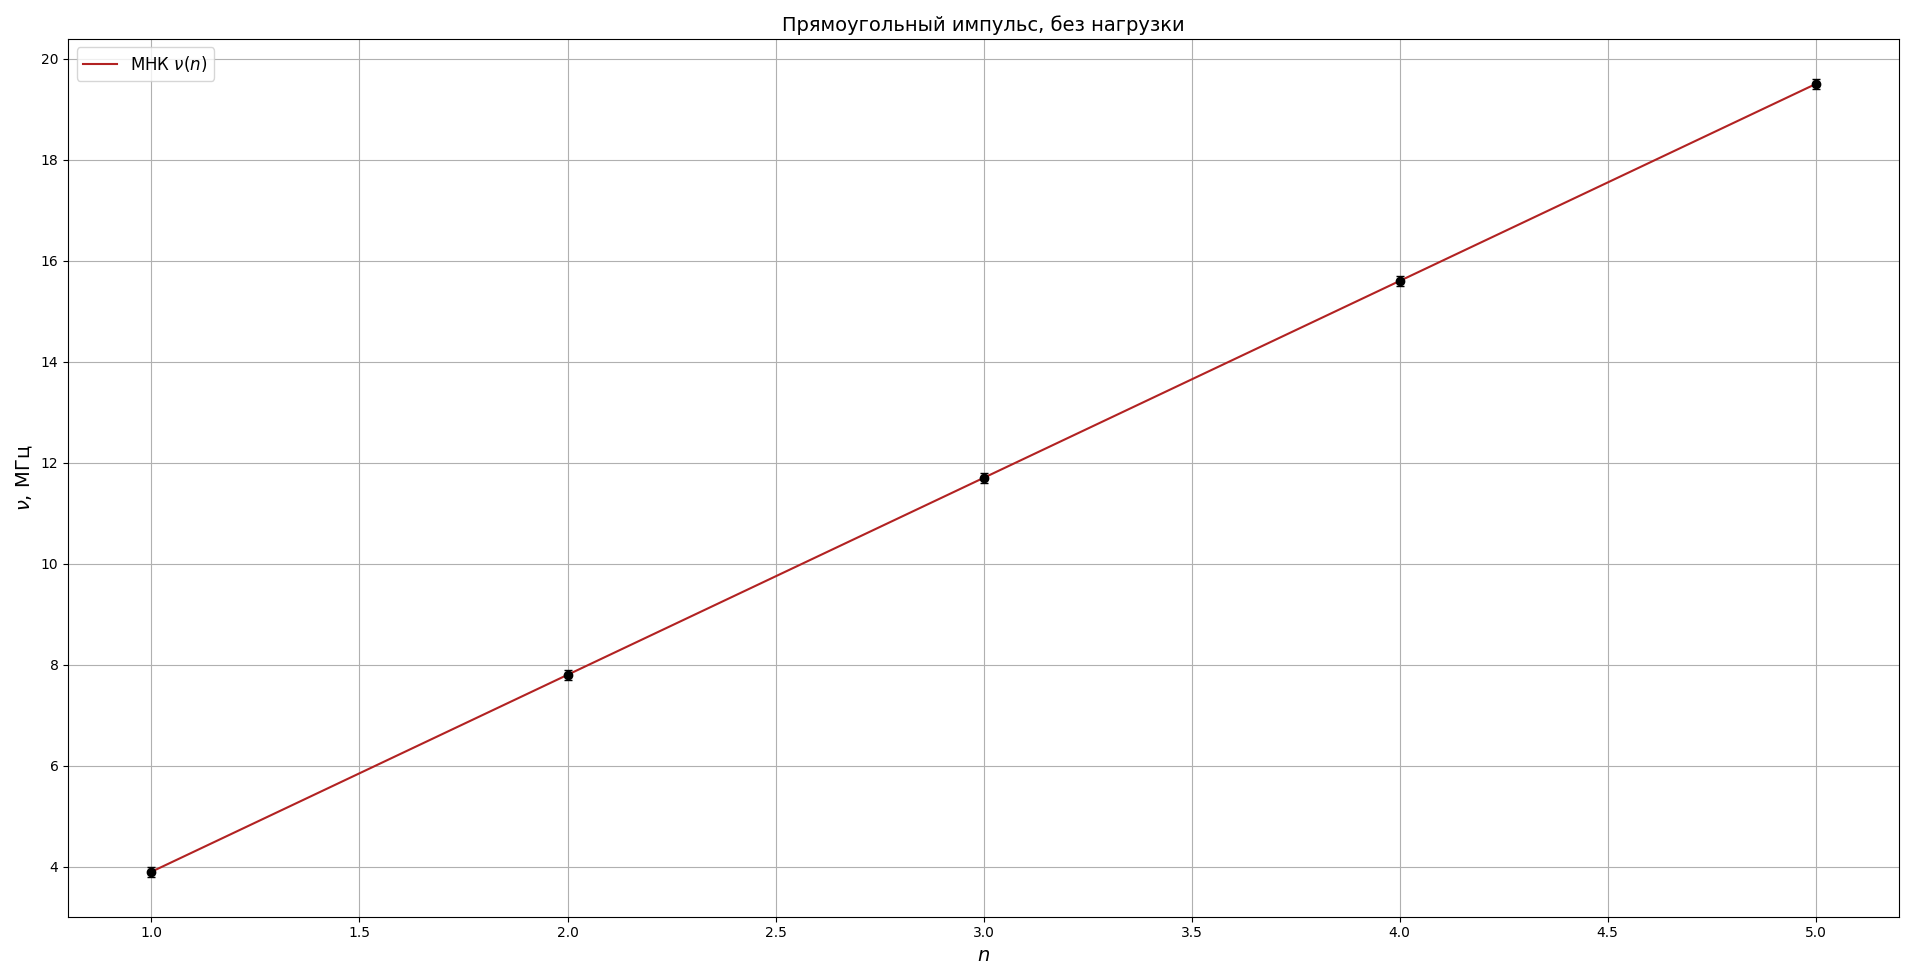
\includegraphics[scale=0.38]{graph32.png}
		\caption{График $\nu(n)$ для прямоугольных сигналов на линии без нагрузки}
	\end{figure}

	Полученный коэффициент наклона прямой
	$$\frac{V_\text{гр}}{l}=3,936\pm0,002\:\text{МГц} $$
	Откуда получим
	$$V_\text{гр}=(1,980\pm0,001)\cdot10^{10}\:\frac{\text{см}}{\text{c}}$$
	
	Групповые скорости измеренные на двух линиях совпали друг c другом с точностью до погрешности. Также групповая скорость с хорошей точностью совпадает с фазовой, что дополнительно свидетельствует об отсутствии дисперсии.
	

	\newpage


	\section{Амплитудно-частотная и фазово-частотная характеристики}

	Снимем зависимости $U_0$, $U_H$, $\Delta \varphi$ от $\nu$. 
	Посчитаем $\omega$, $\alpha(\omega)$ и $k(\omega)$, 
	воспользовавшись формулами (8).

	\begin{table}[h]
		\centering
		\begin{tabular}{|l|l|l|l|l|l|} \hline
			$\nu$, МГц 
					& $2U_{0}$, В 
						   & $2U_{H}$, В 
								  & $\Delta \varphi$ 
								  		  & $\alpha$, $\text{м}^{-1}$  
										           & $k$, $\text{м}^{-1}$ \\ \hline
			1       & 27,1 & 25,2 &  4,62 & 0.0015 & 0.09 \\ \hline
			3       & 27,2 & 24,3 &  7,52 & 0.0023 & 0.15 \\ \hline
			5       & 26,7 & 23,6 & 11,50 & 0.0025 & 0.23 \\ \hline
			7       & 26,7 & 23,4 & 13,74 & 0.0026 & 0.27 \\ \hline
			9       & 27,0 & 22,9 & 16,81 & 0.0033 & 0.34 \\ \hline
			11      & 27,0 & 22,5 & 19,86 & 0.0036 & 0.40 \\ \hline
			13      & 26,9 & 22,0 & 22,94 & 0.0040 & 0.46 \\ \hline
			15      & 27,2 & 21,7 & 25,96 & 0.0045 & 0.52 \\ \hline
			17      & 27,1 & 21,4 & 29,04 & 0.0047 & 0.58 \\ \hline
			20      & 27,1 & 21,4 & 36,66 & 0.0047 & 0.73 \\ \hline
			24      & 27,1 & 21,1 & 42,79 & 0.0050 & 0.85 \\ \hline
			28      & 27,1 & 20,2 & 48,93 & 0.0059 & 0.98 \\ \hline
			32      & 26,8 & 19,7 & 55,01 & 0.0061 & 1.09 \\ \hline
			36      & 26,9 & 19,1 & 61,13 & 0.0068 & 1.22 \\ \hline
			40      & 26,5 & 18,5 & 67,30 & 0.0072 & 1.34 \\ \hline
		\end{tabular}
	\end{table}
	Построим зависимость $y_1(x_1)$, где $x_1=\omega^2$, $y_1=k^2-\alpha^2$
	\newpage
	\begin{figure}[h]
		\centering
		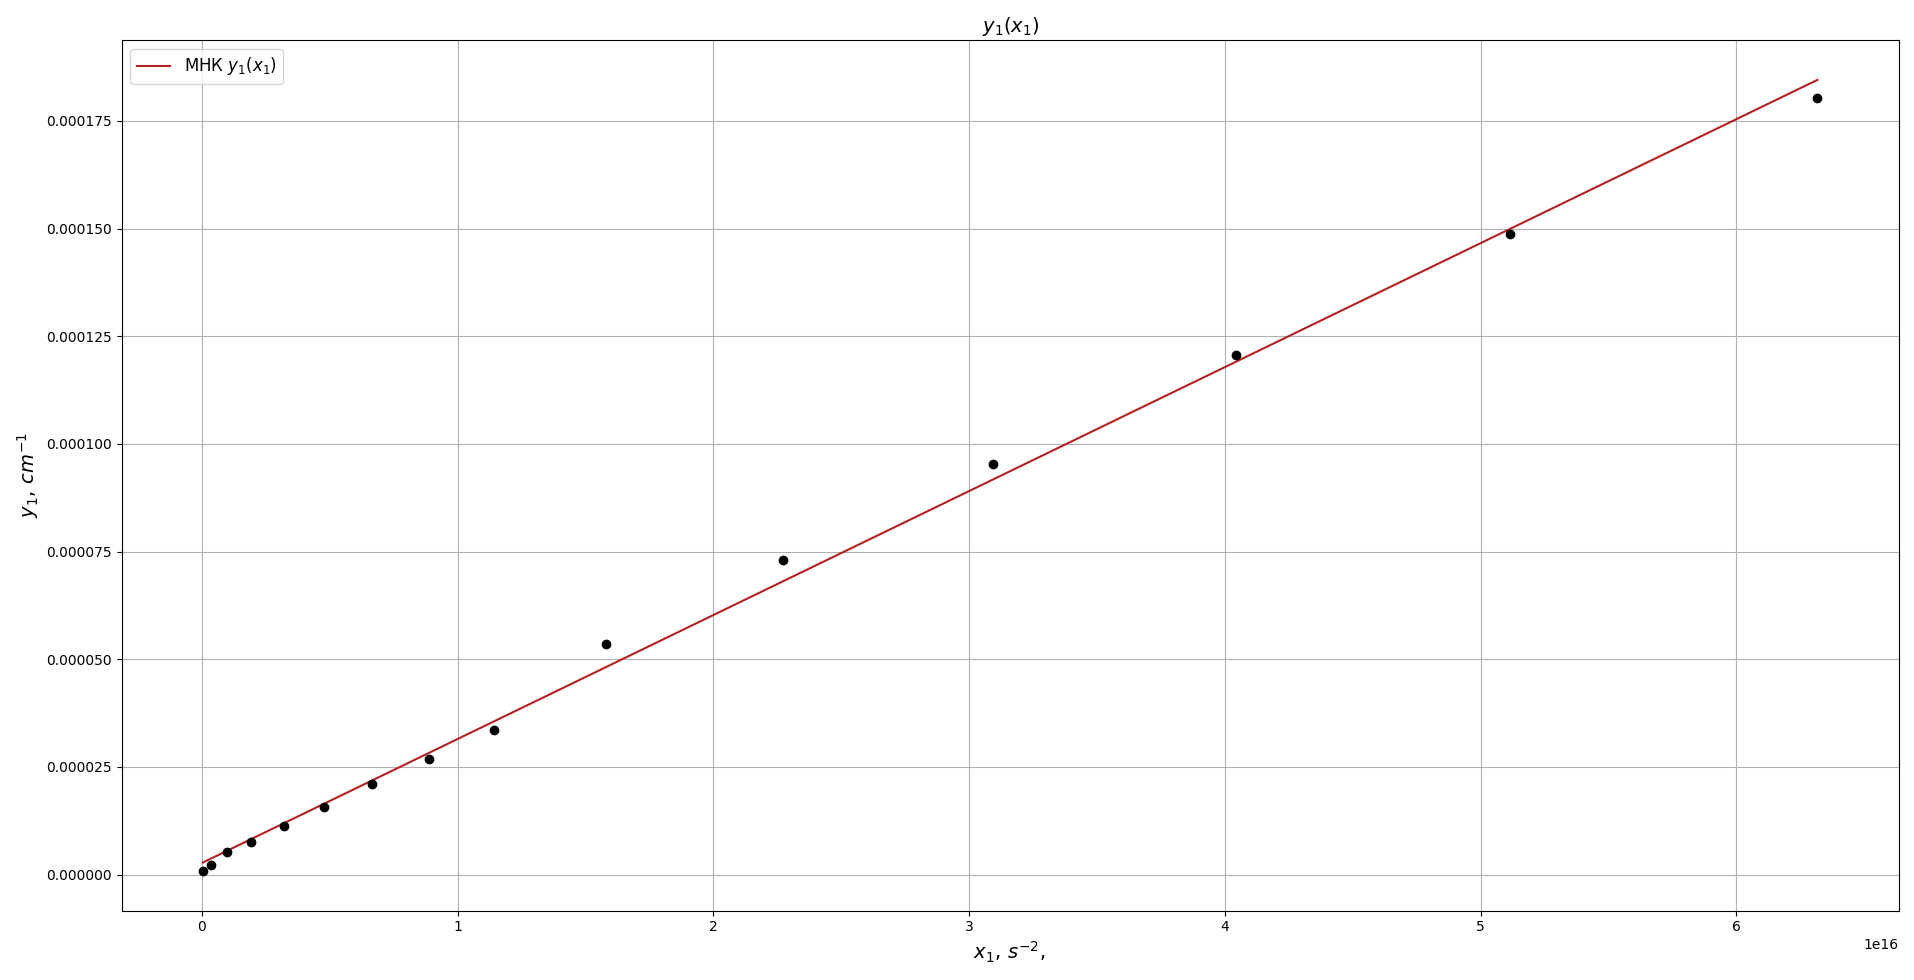
\includegraphics[scale=0.38]{graph41.png}
		\caption{График $y_1(x_1)$}
	\end{figure}

	Полученный коэффициент наклона
	$$\frac{L_xC_x}{c^2}=(2.879\pm0.002)\cdot10^{-21}\:\frac{\text{c}^2}{\text{cм}^2}$$
	Тогда получим
	\begin{equation}
		L_xC_x=2.591\pm0.002
	\end{equation}
	Т.к $R_0=50$ Ом, то согласно (5), получим
	\begin{equation}
		\begin{cases}
			L_x=cR_0\sqrt{L_xC_x} \\
			C_x=\frac{\sqrt{L_xC_x}}{cR_0}
		\end{cases}
	\end{equation}
	Тогда
	\begin{equation}
		L_x=2.414\pm0.001\:\text{ед.СГС}
	\end{equation}
	\begin{equation}
		C_x=1.0731\pm0.0003\:\text{ед.СГС}
	\end{equation}
	Зная это из формул 1 и 2 оценим $\mu$ и $\varepsilon$
	\begin{equation}
		\mu=1.0739\pm0.0004
	\end{equation}
	\begin{equation}
		\varepsilon=2.4122\pm0.0008
	\end{equation}
	Заметим, что $c/\sqrt{\mu\varepsilon}\approx1.87\cdot10^{10}\:\frac{\text{см}}{\text{с}}$, что в пределах некоторой погрешности соответствует ранее измеренной фазовой скорости.
	

	\section{Определение удельной проводимости проводников}
	\subsection{Метод А}
	
	Имеем соотношение
	\begin{equation}
		\alpha = \frac{4}{\sqrt{\sigma} d}C_x\frac{V_\text{ф}}{c}\sqrt{\nu}+\alpha_0
	\end{equation}
	где $\alpha_0$ -- поправочный коэффициент. Построим зависимость $y_2(x_2)$, где $y_2=\alpha$, $x_2=\sqrt{\nu}$.
	
	Полученное значение коэффициента наклона
	\begin{equation}
		a=\frac{4}{\sqrt{\sigma} d}C_x\frac{V_\text{ф}}{c}=(1.07\pm0,03)\cdot10^{-8}\:\text{см}\cdot\text{c}^{1/2}
	\end{equation}

	Отсюда получим
	\begin{equation}
		\sigma_1 = \left(\frac{4C_xV_\text{ф}}{acd}\right)^2=(4.02\pm0.08)\cdot10^{18}\:\text{ед.СГС}
	\end{equation}
	
	\begin{figure}[h]
		\centering
		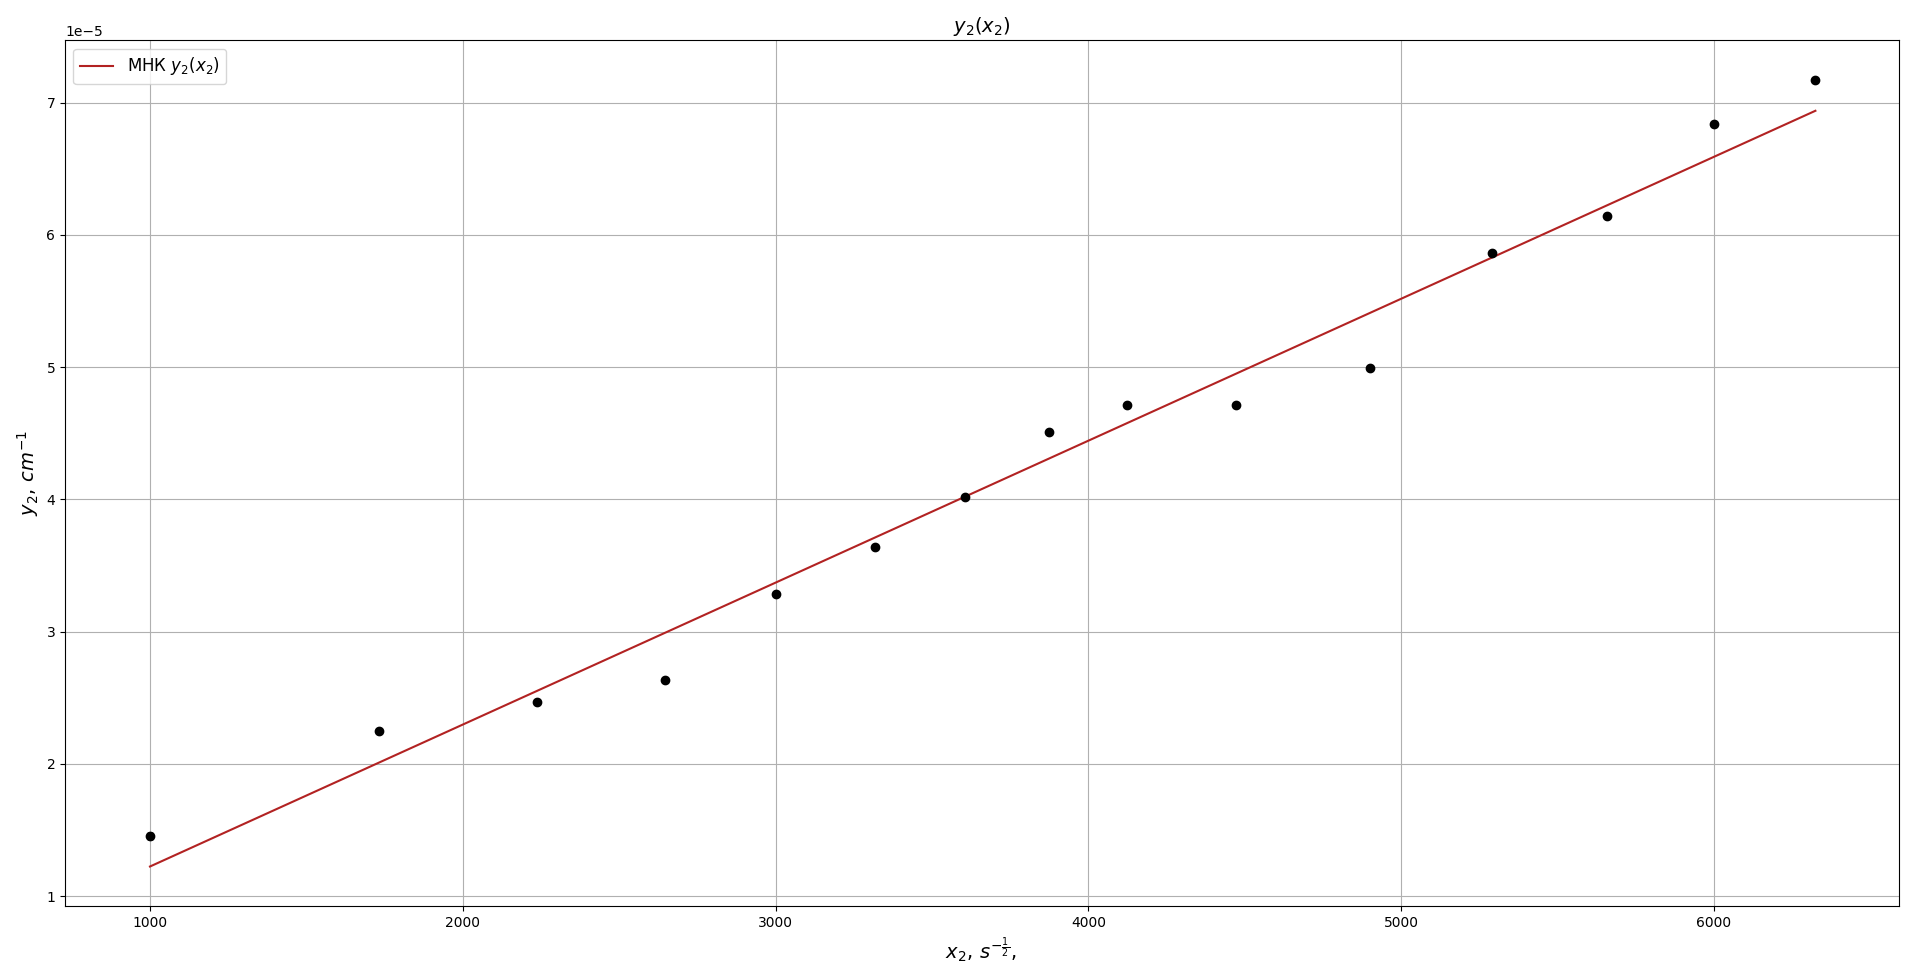
\includegraphics[scale=0.38]{graph51.png}
		\caption{График $y_2(x_2)$}
	\end{figure}
	
	\subsection{Метод Б}
	Из теории известно, что 
	\begin{equation}
		2\alpha k=\omega R_xC_x
	\end{equation}
	Которое можно свести к зависимости
	\begin{equation}
		y_3=\frac{4\pi C_x}{cd\sqrt{\sigma}}x_3
	\end{equation}
	где $x_3=\nu^{3/2}$, $y_3=\alpha k$.
	\begin{figure}[h]
		\centering
		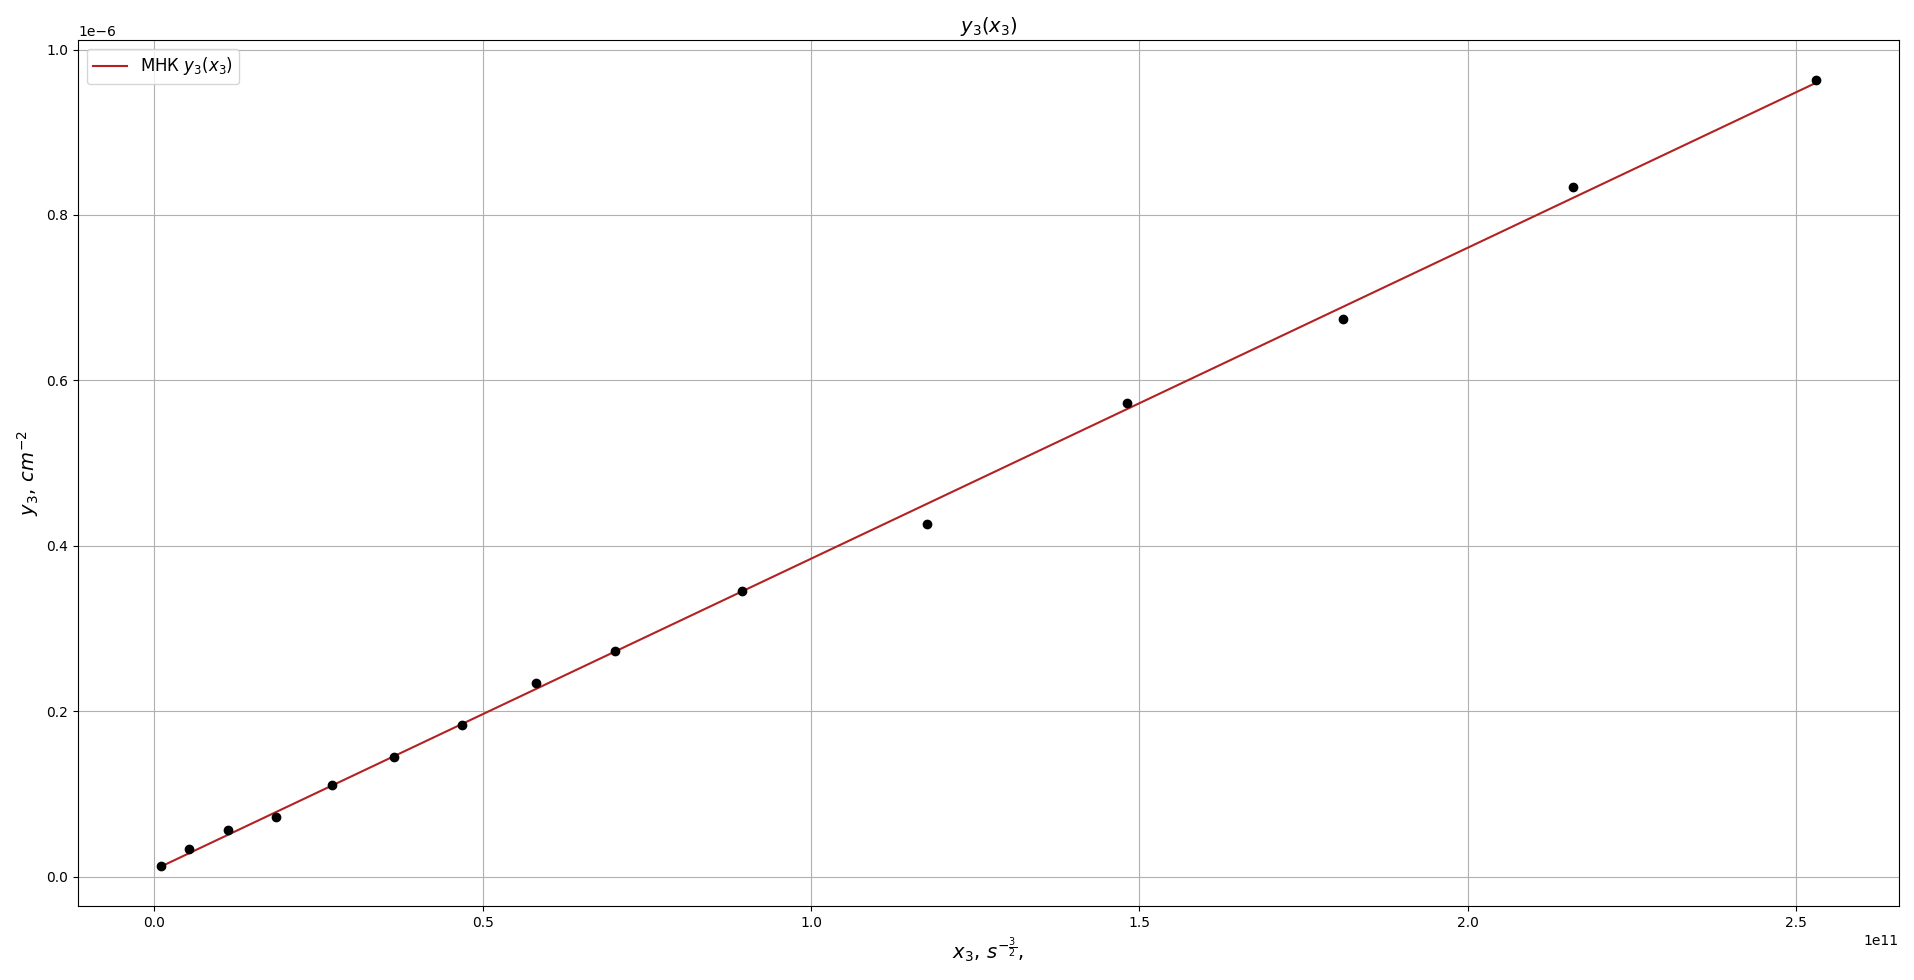
\includegraphics[scale=0.38]{graph52.png}
		\caption{График $y_3(x_3)$}
	\end{figure}

	Полученное значение коэффициента наклона
	\[a=\frac{4\pi C_x}{cd\sqrt{\sigma}}=(3.76\pm0.02)\cdot10^{-18}\:\text{ед.СГС}\]
	Отсюда получим
	\begin{equation}
		\sigma_2=\left(\frac{4\pi C_x}{acd}\right)^2=(8.46\pm0.05)\cdot10^{17}\:\text{ед.СГС}
	\end{equation}

	\section{Вывод}
	
	Была измерена фазовая скорость. Для согласованной и отсутствующей нагрузок
	они соответственно равны:
	\[V_\text{Ф}=(1,953\pm0,001)\cdot10^{10}\:\frac{\text{см}}{\text{с}}\]
	\[V_\text{Ф}=(1,943\pm0,002)\cdot10^{10}\:\frac{\text{см}}{\text{с}}\]
	и групповые скорости для согласованной и отсутствующей нагрузок:
	\[V_\text{гр}=(1,954\pm0,001)\cdot10^{10}\:\frac{\text{см}}{\text{c}}\]
	\[V_\text{гр}=(1,980\pm0,001)\cdot10^{10}\:\frac{\text{см}}{\text{c}}\]
	Получили, что групповая скорость с хорошей точностью совпадает с фазовой, что свидетельствует об отсутствии дисперсии.
	
	Далее были сняты амплитудно-частотная и фазово-частотная характеристики. Была построена зависимость $y_1(x_1)$, по которой было определено произведение $L_xC_x$. Отсюда были получены погонные характеристики
	\begin{equation*}
		L_x=2,414\pm0,001\:\text{ед.СГС}
	\end{equation*}
	\begin{equation*}
		C_x=1,0731\pm0,0003\:\text{ед.СГС}
	\end{equation*}
	и характеристики среды
	\begin{equation*}
		\mu=1,0739\pm0,0004
	\end{equation*}
	\begin{equation*}
		\varepsilon=2,4122\pm0,0008
	\end{equation*}
	Значение фазовой скорости, вычисленное через характеристики среды с неплохой точностью ($~5\%$)совпало с ранее вычисленным значением.
	
	Далее методами А и Б была вычислена проводимость. Для методов А и Б значения проводимости соответственно равны
	\begin{equation*}
		\sigma_1 =(4,02\pm0,08)\cdot10^{18}\:\text{ед.СГС}
	\end{equation*}
	\begin{equation*}
		\sigma_2=(8,46\pm0,05)\cdot10^{17}\:\text{ед.СГС}
	\end{equation*}
	Отличие в 5 раз может объясняться тем, что амплитудная характеристика была измерена с ошибками, что оказало влияние на результаты обработки. В методе А была попытка вычислить константу, на которую отличаются измерения, однако, очевидно, точность такой корректировки по прежнему недостаточна.
\end{document}